\chapter{SALSA-hemsidan}
SALSA-teleskopen har en hemsida som du når via {\bf
http://vale.oso.chalmers.se/salsa}, en del av sidan kan ses i Fig.
\ref{fig:website}. Här hittar du användbar information och mjukvara som kan
hjälpa dig att använda teleskopet och analysera mätdata. 
\begin{figure}[h]
\centering
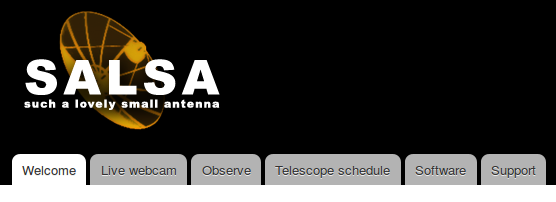
\includegraphics[width=\textwidth]{../figures/SALSA_website.png}
\caption{\label{fig:website} En del av SALSA-hemsidan. Här finns mycket
användbar information och även bokningssystemet som används för att reservera
observationstid med SALSA.}
\end{figure}

\section{Skapa ett konto}
För att styra SALSA så måste du först skapa ett användarkonto på SALSA-hemsidan. 
Om du inte redan gjort deta, leta upp länken \emph{Create new account} 
och fill i dina uppgifter. Du bör nu få en bekräftelse med login-information 
via email, om inte - kolla så att mailet inte hamnat i skräppost. 

\section{Boka teleskoptid}
För att kunna observera så måste du först boka tid. Detta krävs eftersom
endast en användare kan använda teleskopet åt gången. Bokningar görs via 
SALSA-hemsidan. När du är inloggad, gå till sidan \emph{Observe}. På denna sida
så finns en länk \emph{Book a time}. Klicka här för att skapa en ny bokning. 
En ny sida visas nu där du måste fylla i en kort beskrivning av din observation,
se Fig. \ref{fig:book}.
\begin{figure}[h]
\centering
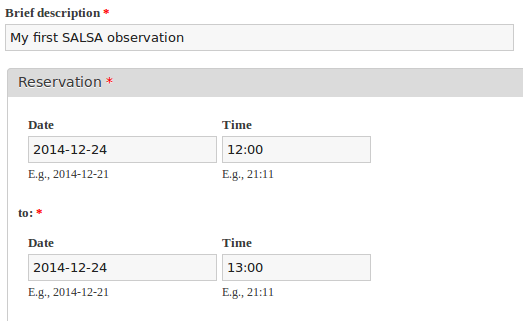
\includegraphics[width=\textwidth]{../figures/SALSA_book.png}
\caption{\label{fig:book} Sidan som används för att skapa en ny bokning av 
	observationstid med SALSA.}
\end{figure}

Därefter väljer du start- och sluttid för din observation. Du kan kolla på sidan
\emph{Telescope schedule} för att hitta en ledig tid. Observera att du kan klicka
i datum-fälten för att få en pop-up-kalender där du kan välja datum. 
Tids-fälten anger timmar och minuter på den dag du valt. Du kan växla mellan att 
ändra timmmar eller minuter genom att klicka med musen i fältet, eller genom
att använda piltangenterna på ditt tangentbord. Observera att tiderna anges
i den tidszon du valt när du registrerade dig. (Om du vill kontrollera
din tidszon, klicka på länken \emph{My account}.)

Till sist måste du välja ett teleskop. Vi gör vårt bästa för att se till att 
det alltid finns minst ett teleskop tillgängligt, ibland finns det två eller t.o.m.
tre att välja på. De kan bokas oberoende av varandra, så om ett teleskop är bokat
under en viss tid så kan du prova att boka ett annat. Välj minst ett teleskop
och klicka sedan på \emph{Save} för att spara din bokning. Du bör nu se din bokning
på sidan \emph{My reservations}, och även på sidan \emph{Telescope
schedule}. 

Nu kan du styra teleskopet under den tid du bokat. Observera att du inte kan
använda teleskopet om du inte har bokat. Notera också att om din bokning tar
slut under tiden som du använder teleskopet, då kommer dina observationer
att avslutas och kontrollprogrammet stängas ner. Därför är det bra att spara 
din data under tiden du observerar, se nedan. Om du inser under din bokade tid
att du behöver mer tid, då kan du prova att förlänga din bokning. Detta kan du göra
genom att gå in på sidan \emph{My reservations} och klicka på länken 
\emph{edit} för att ändra en specifik bokning.

\section{Live webkamera}
Det är roligare att styra teleskop om du kan se dem röra sig! Därför har vi 
monterat en webbkamera i en byggnad nära teleskopen. Du kommer åt webkameran
via sidan \emph{Live webcam} på SALSA-hemsidan.

\section{Webarkiv för mätdata}
\label{sect:archive}
När du gjort en mätning med SALSA så kan du ladda upp den till webarkivet. För
att komma åt din arkiverade data, logga in på SALSA-hemsidan och klicka på länken 
\emph{Data archive}. Denna sida visar ditt personliga arkiv, alltså alla dina 
sparade mätdata. Varje mätning kan laddas ner som tre olika format: som PNG 
(en bild, praktiskt för en snabbtidd på din mätning), som TXT (en ren textfil
med rådatan), och som FITS (ett vanligt format inom astronomi
för att analysera mätningar i detalj). Instruktioner för hur du läser
dessa olika format finns i avsnitt \ref{sect:archiveprocess} i detta dokument.
\begin{figure}[h]
\centering
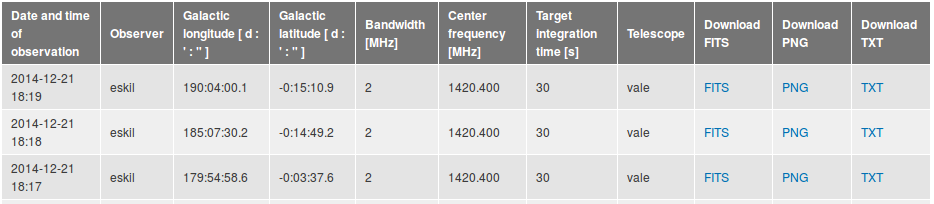
\includegraphics[width=\textwidth]{../figures/SALSA_archive.png}
\end{figure}
